\documentclass[10pt,a4paper,twocolumn]{article}
\usepackage[utf8]{inputenc}
\usepackage{amsmath}
\usepackage{amsfonts}
\usepackage{amssymb}
\usepackage{graphicx}
\usepackage{url}
\usepackage{chato-notes}

\author{Igo Ramalho Brilhante \\ \small{Universidade Federal do Ceará} \\  \small{\textit{igobrilhante@lia.ufc.br}} \and Tales Parente \\  \small{Universidade Federal do Ceará} \\ \small{\textit{talespf@lia.ufc.br}} }
\title{Projeto RecomendAI}

\begin{document}

\maketitle

\section{Proposta de Projeto}

\subsection{Motivação}
Escolher os locais a serem visitados quando se planeja uma viagem turística pode ser uma tarefa nem sempre fácil de ser executada, principalmente quando se visita uma cidade pela primeira vez. Descobrir uma atração turística ou um restaurante para os momentos de descanso que sejam próximos ao local onde se encontram é uma situação comum para turistas e, geralmente, requer planejamento por parte de quem viaja.

Fortaleza é uma cidade que vem sediando cada vez mais eventos de grande porte e é esperado um grande fluxo de turistas para os próximos anos. Diante desse cenário, é interesante que o turista possa contar com meios que o auxiliem a melhor explorar a cidade. A exploração de locais na cidade, ainda, pode ser feita pelos habitantes da cidade, embora estes já tenham mais conhecimento sobre a mesma.

Obviamente que recomendar pontos de interesses não é um tarefa simples uma vez que muitas variáveis podem ser ou devem ser consideradas, como tempo e espaço. Para realizar recomendações mais efetivas é necessário, portanto, considerar o momento no qual o usuário se encontra. Para isso, o \emph{contexto} no qual o usuário está inserido é levado em consideração. Contexto aqui considera-se a atual posição geográfica (latitude e longitude), o dia da semana, a hora do dia e as condições climáticas no qual o usuário se encontra.

\subsection{Problema}
Dado o cenário acima, auxiliar turistas e habitantes da cidade de Fortaleza sugerindo uma lista de atrações turísticas na cidade de Fortaleza, levando em conta o contexto (espacial e temporal) em que ele está inserido.
	
\subsection{Proposta}
Desenvolver uma aplicação para dispositivos móveis com sensibilidade ao contexto que auxilie na exploração de pontos de interesses da cidade de Fortaleza. A aplicação deve recomendar uma lista de atrações ou pontos de interesses que o usuário pode visitar, levando em consideração informações relativas à atual localização geográfica do usuário, o dia da semana, a hora do dia e as condições climáticas no instante de tempo. A ideia é que o usuário possa ter sugestões do próximo local a visitar (museu, monumento, restaurante etc.) dado o o contexto no qual o usuário se encontra. Figura \ref{fig:visao_geral} mostra a visão geral da proposta, onde o usuário dentro de um certo contexto é auxiliado pela aplicação para a descoberta de pontos de interesses a serem visitados a partir da sua atual posição geográfica.

\begin{figure}[!hbt]
\centering
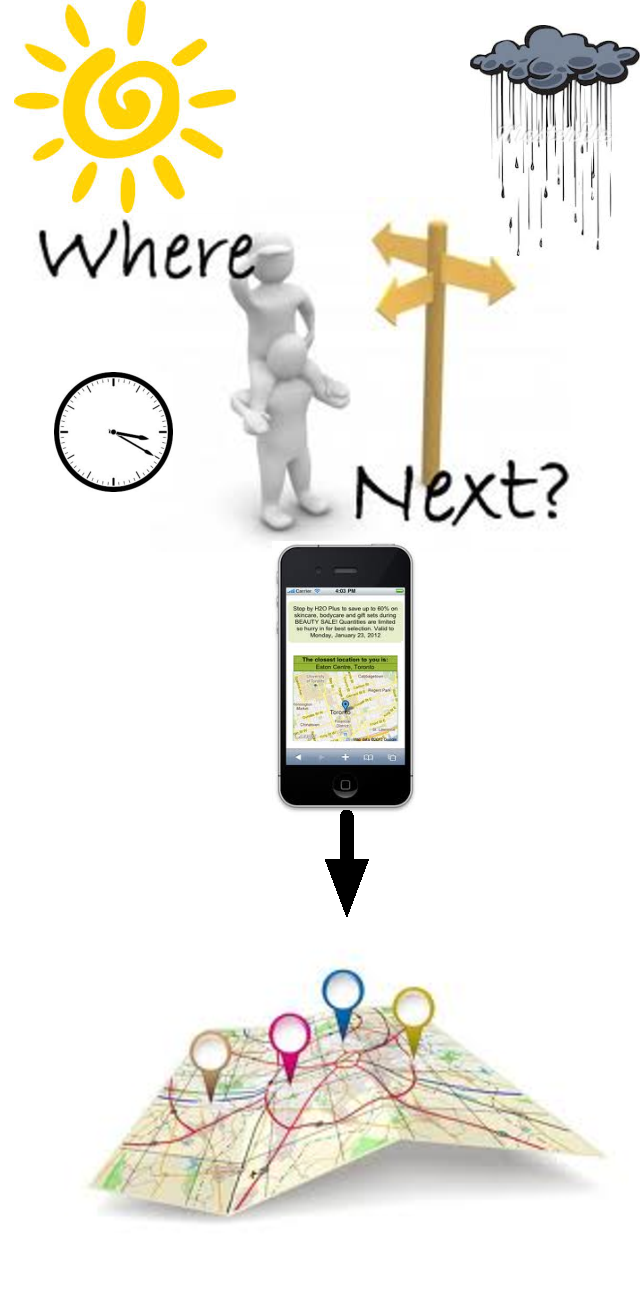
\includegraphics[scale=0.25]{figuras/exemplo.pdf}
\caption{Visão geral da proposta}
\label{fig:visao_geral}
\end{figure}

\begin{enumerate}
\item Público alvo: turistas e habitantes da cidade de Fortaleza
\item Aplicação Cliente
\begin{enumerate}
\item Tecnologia: Plataforma Android \cite{Android}
\end{enumerate}
\item Servidor
\begin{enumerate}
\item Algoritmo de recomendação para o próximo local
\item Pontos de interesses oferecidos pelo Foursquare \cite{Foursquare}
\end{enumerate}

\end{enumerate}




\bibliographystyle{plain}
\bibliography{biblio}
\end{document}